\documentclass[border=10pt]{standalone}
\usepackage{pgfplots}
\pgfplotsset{compat=1.18}
\begin{document}
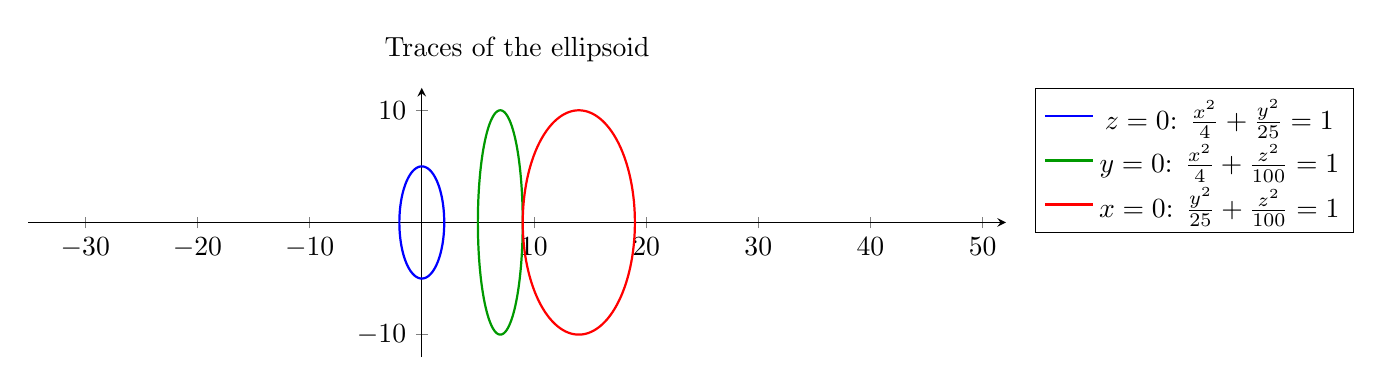
\begin{tikzpicture}
\begin{axis}[
    width=14cm, height=5cm,
    axis equal,
    axis lines=middle,
    enlargelimits=true,
    title={Traces of the ellipsoid},
    legend pos=outer north east
]
\addplot[blue, thick, domain=0:360, samples=200, variable=\t]
({2*cos(\t)}, {5*sin(\t)});
\addplot[green!60!black, thick, domain=0:360, samples=200, variable=\t]
({2*cos(\t)+7}, {10*sin(\t)});
\addplot[red, thick, domain=0:360, samples=200, variable=\t]
({5*cos(\t)+14}, {10*sin(\t)});
\legend{$z=0$: $\frac{x^2}{4}+\frac{y^2}{25}=1$,
        $y=0$: $\frac{x^2}{4}+\frac{z^2}{100}=1$,
        $x=0$: $\frac{y^2}{25}+\frac{z^2}{100}=1$}
\end{axis}
\end{tikzpicture}
\end{document}
